% Copyright 2020 by Junwei Wang <i.junwei.wang@gmail.com>
%
% This file may be distributed and/or modified under the
% conditions of the LaTeX Project Public License, either version 1.3c
% of this license or (at your option) any later version.
% The latest version of this license is in
%   http://www.latex-project.org/lppl.txt

\documentclass[compress]{beamer}
\usepackage[english]{babel}
\usepackage{metalogo}
\usepackage{listings}
\usepackage{fontspec}
\usepackage{tikz}
\usepackage{graphicx}
\usepackage{minted}

\graphicspath{ {./pictures/} }

% \usetheme{Nord}
\usetheme[style=light]{Nord}


\setmainfont{DejaVu Sans Mono}
\setsansfont{DejaVu Sans Mono}
\setmonofont{DejaVu Sans Mono}

\AtBeginSection[]
{
  \begin{frame}[c,noframenumbering,plain]
    \tableofcontents[sectionstyle=show/hide,subsectionstyle=show/show/hide]
  \end{frame}
}

\AtBeginSubsection[]
{
  \begin{frame}[c,noframenumbering,plain]
    \tableofcontents[sectionstyle=show/hide,subsectionstyle=show/shaded/hide]
  \end{frame}
}

\title{Building a Wall Detecting Robot}
\author{Jack Robbers}
\institute{CREATE UNSW}
\date{\today}

\begin{document}

\begin{frame}[plain,noframenumbering]
  \maketitle
  Table of Contents:
  \tableofcontents
\end{frame}

\section{Introduction}

\begin{frame}[fragile]
    \frametitle{Who are you?}
    Jack Robbers (he/him)
    \begin{itemize}
        \item 2nd Year Electrical Engineering and Computer Science Student at UNSW
        \item Currently doing an internship making sensors for robots
        \item Ask me about robots, web dev, uni or any questions you have during the workshop
    \end{itemize}

    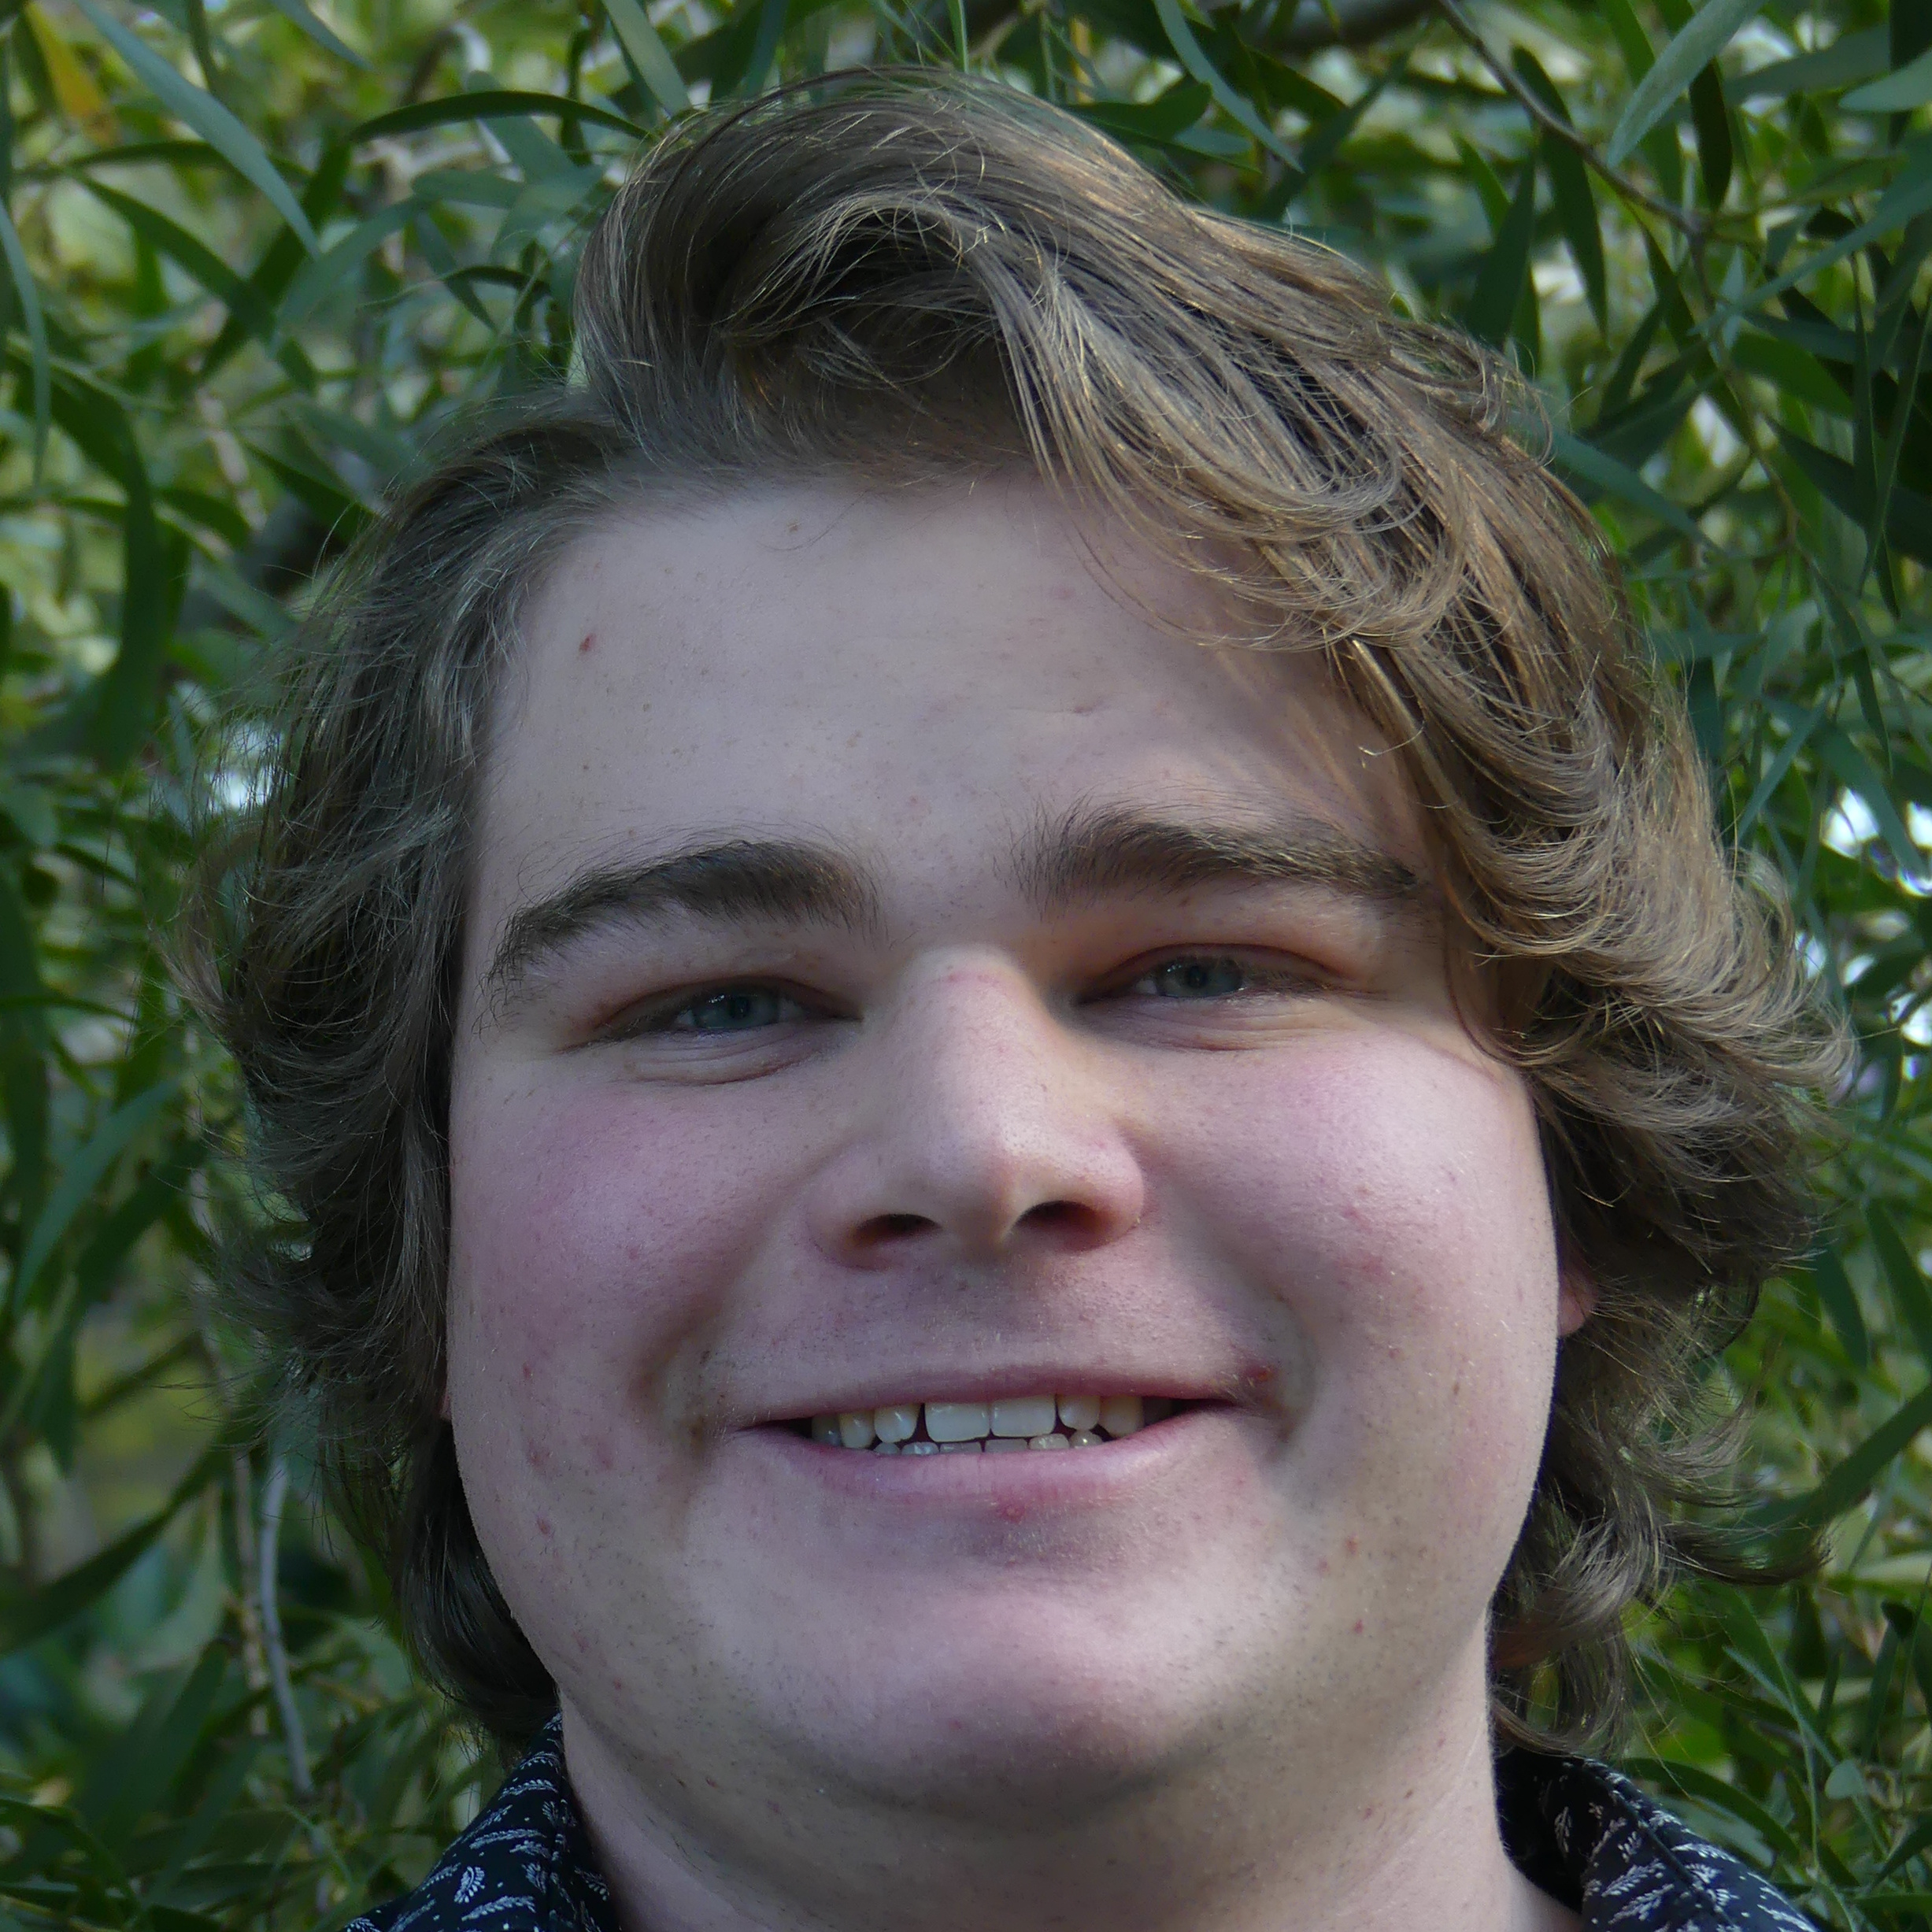
\includegraphics[height=5cm]{pictures/jack.jpg}
\end{frame}

\section{Electronics and Circuity}

\begin{frame}[fragile]
    \frametitle{What's in the kit?}
    \begin{itemize}
        \item <1-> {\color{NordRed}Wheels}
        \item <2-> {\color{NordRed}Motors}
        \item <3-> {\color{NordRed}Jumper Wires (Plug-Socket \& Plug-Plug)}
        \item <4-> {\color{NordRed} Aligator Clips}
        \item <5-> {\color{NordRed} Arduino (and USB cable)}
        \item <6-> {\color{NordRed} Breadboard}
        \item <7-> {\color{NordRed} Resistors}
        \item <8-> Potentiometer
        \item <9-> {\color{NordRed}Ultrasonic Sensor}
        \item <10-> LEDs (Clear, Coloured, and RGB)
        \item <11-> Slide Switch
        \item <12-> Buzzer
        \item <13-> Phototransistor
        \item <14-> Light Dependent resistor
        \item <15-> Transistor
        \item <16-> {\color{NordRed}Motor driver and screwdriver}
    \end{itemize}
\end{frame}

\begin{frame}[fragile]
    \frametitle{Building the Circuit}
    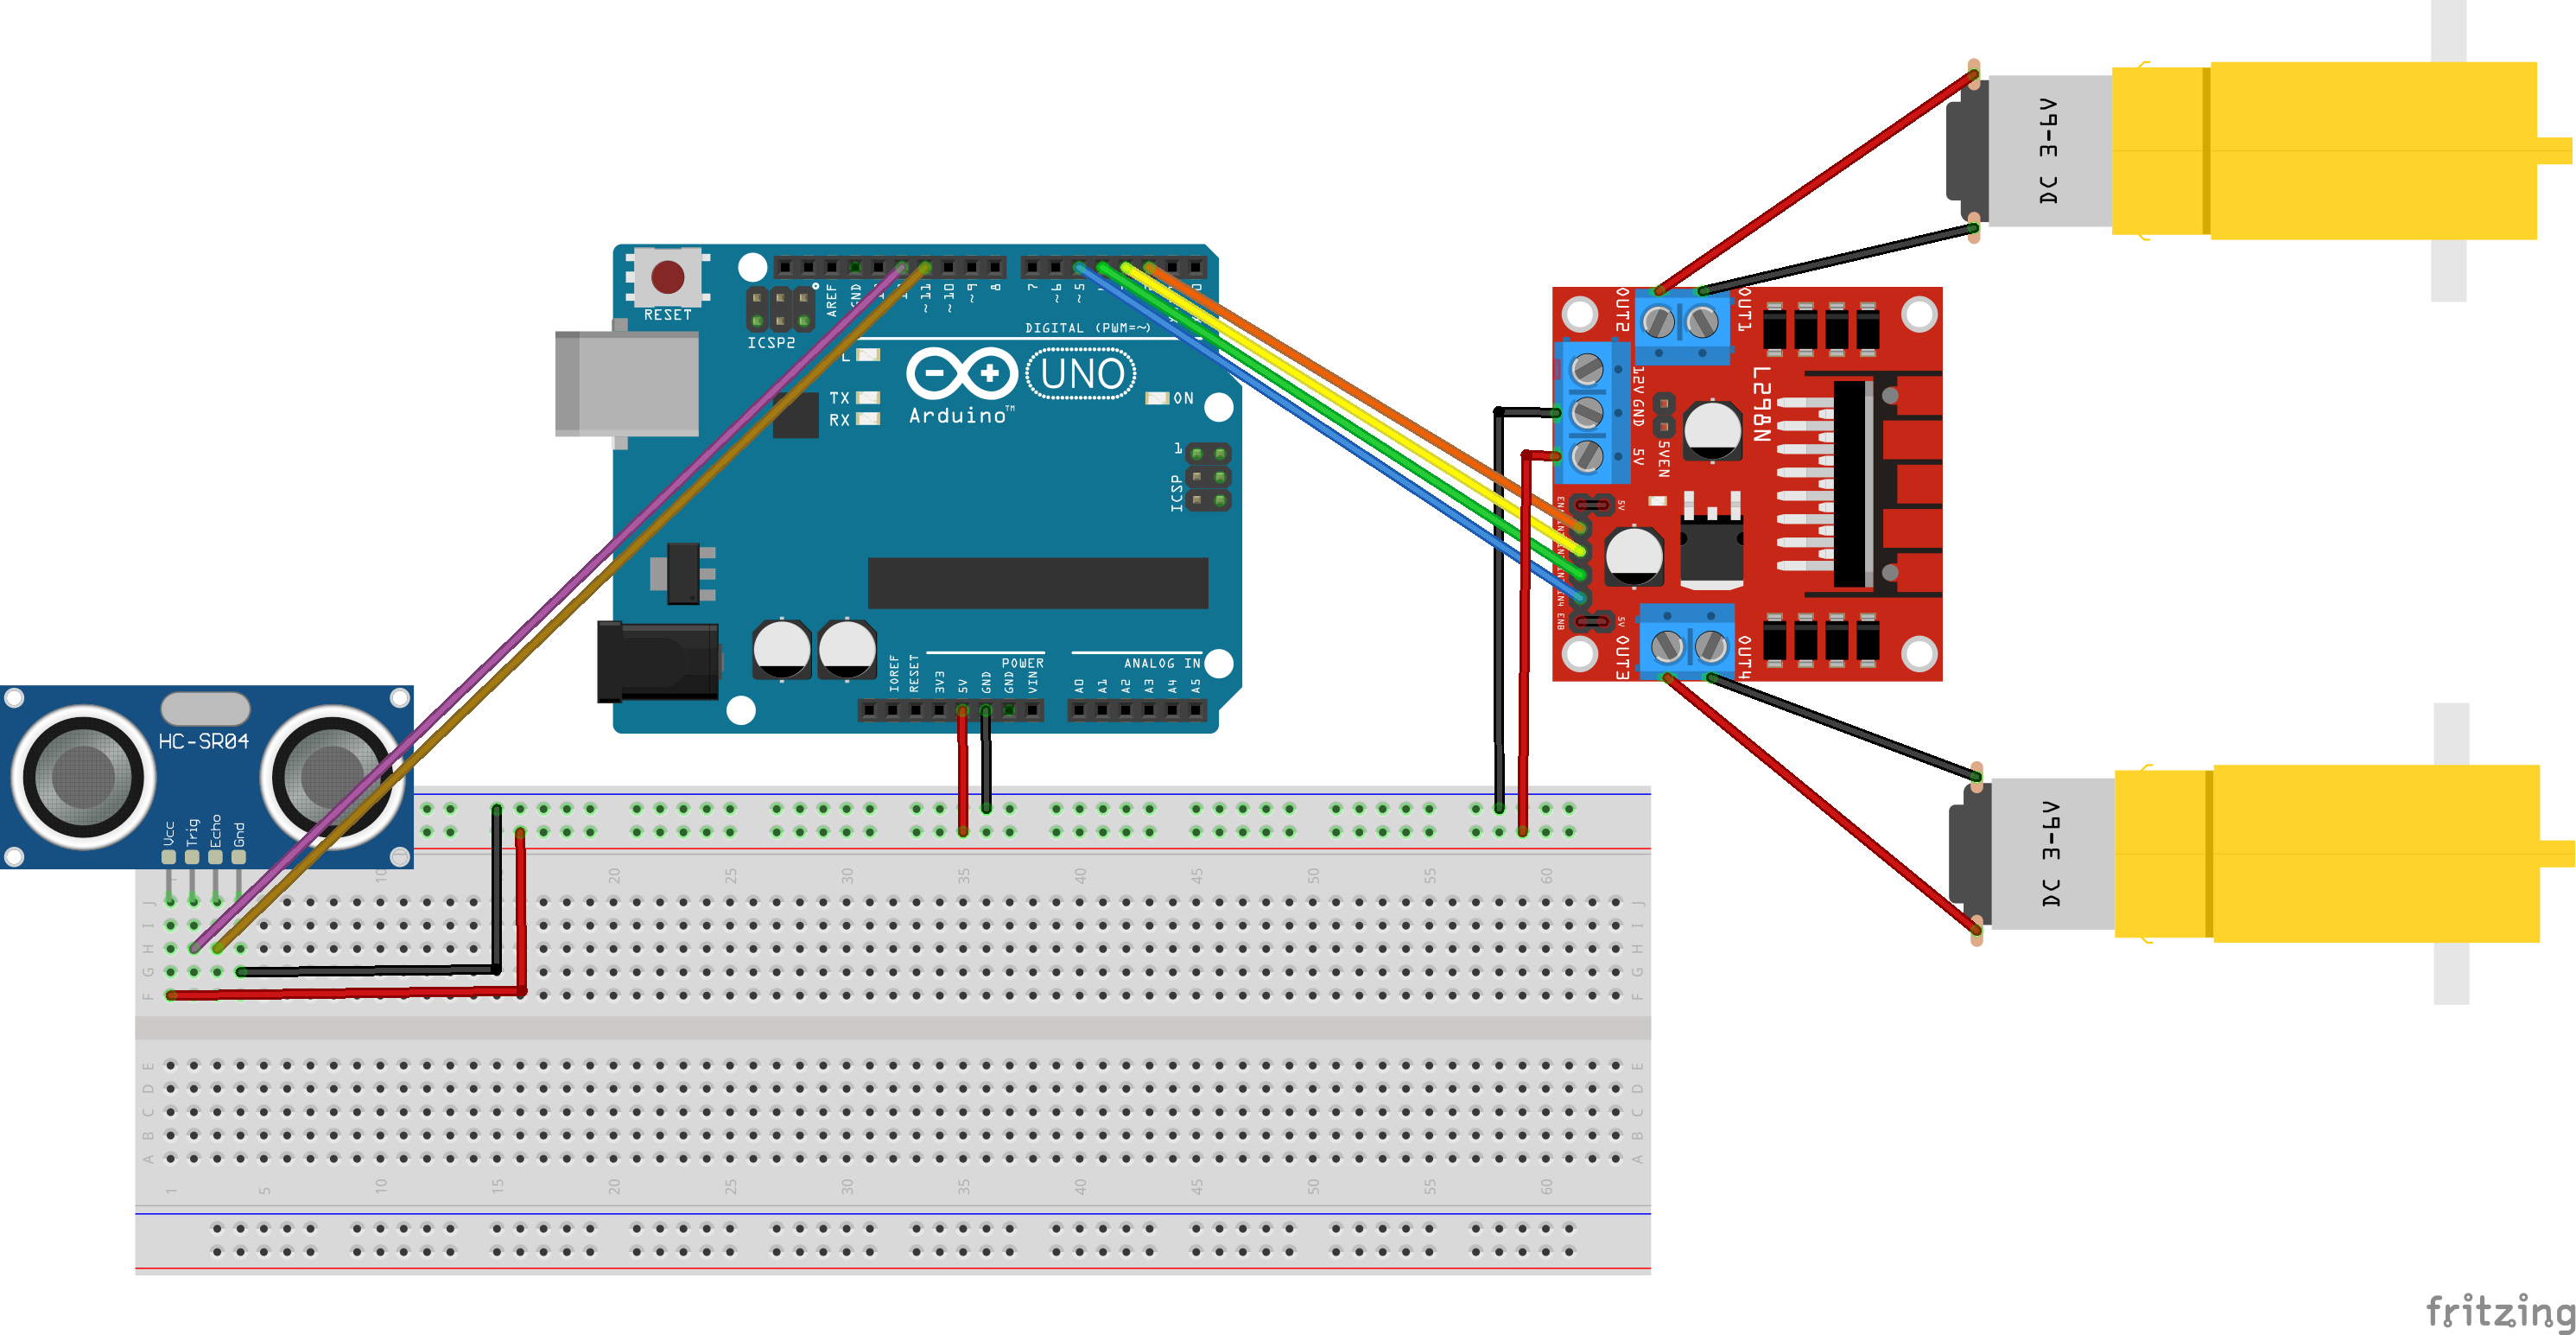
\includegraphics[height=7cm]{pictures/circuit.png}
\end{frame}

\section{Programming}

\begin{frame}[fragile]
    \inputminted[linenos, breaklines, firstline=1, lastline=10]{arduino}{code/workshop.ino}
\end{frame}

\begin{frame}[fragile]
    \inputminted[linenos, breaklines, firstline=11, lastline=24]{arduino}{code/workshop.ino}
\end{frame}

\begin{frame}[fragile]
    \inputminted[linenos, breaklines, firstline=25, lastline=38]{arduino}{code/workshop.ino}
\end{frame}

\begin{frame}[fragile]
    \inputminted[linenos, breaklines, firstline=39, lastline=45]{arduino}{code/workshop.ino}
\end{frame}

\begin{frame}[fragile]
    \inputminted[linenos, breaklines, firstline=46, lastline=61]{arduino}{code/workshop.ino}
\end{frame}

\section{Summary}

\begin{frame}[fragile]
    \frametitle{Resources}
    \begin{itemize}
        \item \href{https://howtomechatronics.com/tutorials/arduino/arduino-dc-motor-control-tutorial-l298n-pwm-h-bridge/}{Howto Mechatronics Motor Driver Tutorial}
        \item \href{https://howtomechatronics.com/tutorials/arduino/ultrasonic-sensor-hc-sr04/}{Howto Mechatronics Ultrasonic Sensor Tutorial}
        \item \href{https://www.createunsw.com.au/}{Create Website}
        \item \href{https://www.arduino.cc/reference/en/}{Arduino Reference}
    \end{itemize}
\end{frame}

\begin{frame}[fragile]
    \frametitle{Questions?}
\end{frame}

\end{document}

%%% Local Variables:
%%% mode: latex
%%% TeX-master: t
%%% TeX-engine: xetex
%%% End:
